\documentclass{article}
\usepackage[margin=1in]{geometry}
\usepackage{amsmath,amsthm,amssymb}
\usepackage{bbm,enumerate,mathtools}
\usepackage{tikz,pgfplots}
\usepackage{chessboard}
\usepackage[hidelinks]{hyperref}
\usepackage{multicol} % Problem 35

\newenvironment{question}{\begin{trivlist}\item[\textbf{Question.}]}{\end{trivlist}}
\newenvironment{note}{\begin{trivlist}\item[\textbf{Note.}]}{\end{trivlist}}
\newenvironment{references}{\begin{trivlist}\item[\textbf{References.}]}{\end{trivlist}}
\newenvironment{related}{\begin{trivlist}\item[\textbf{Related.}]\end{trivlist}\begin{enumerate}}{\end{enumerate}}


\begin{document}
Consider all rectangles with all corners on gridpoints on an $n \times m$ grid.
\begin{figure}[!h]
  \centering
  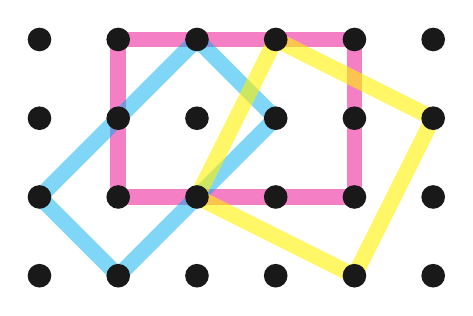
\begin{tikzpicture}
    \draw[magenta, opacity=0.5, line width=0.2cm] (5,4)--(2,4)--(2,2)--(5,2)--cycle;
    \draw[cyan, opacity=0.5, line width=0.2cm]  (1,2)--(3,4)--(4,3)--(2,1)--cycle;
    \draw[yellow, opacity=0.6, line width=0.2cm]  (3,2)--(4,4)--(6,3)--(5,1)--cycle;
    \foreach \x in {1,...,6} {
      \foreach \y in {1,...,4} { \fill[black!90] (\x,\y) circle (0.15cm); }
    }
  \end{tikzpicture}
  \caption{
    An example of three rectangles with all corners on gridpoints of a
    $4 \times 6$ grid.
  }
\end{figure}

\begin{question}
  How many such rectangles exist?
\end{question}
\begin{related}
  \item How many squares exist? Rhombuses? Parallelograms? Kites? Quadrilaterals?
  \item What if we want to count only ``primitive'' squares, in the sense that
    the sides of the square only intersect gridpoints at the corners?
  \item Number of rectangles on the cylinder? Torus? M\"obius strip?
    % \\ % Cylinder
    % \begin{tikzpicture}[scale=0.5]
    %   \draw[magenta, opacity=0.5, line width=0.1cm] (8,3)--(6,4)--(4,5)--(3,3)--(5,2)--(7,1)--(8,0.5);
    %   \draw[magenta, opacity=0.5, line width=0.1cm] (1,3)--(3,2)--(2,0)--(1,0.5);
    %   % \draw[cyan, opacity=0.5, line width=0.2cm]  (1,2)--(3,4)--(4,3)--(2,1)--cycle;
    %   % \draw[yellow, opacity=0.6, line width=0.2cm]  (3,2)--(4,4)--(6,3)--(5,1)--cycle;
    %   \foreach \x in {1,...,8} {
    %     \foreach \y in {0,...,5} { \fill[black!90] (\x,\y) circle (0.15cm); }
    %   }
    % \end{tikzpicture}
  \item Number of ``rotation classes'', where two squares are equivalent if
    one can be transformed into the other by shifting and stretching?
  \item Number of ``orientation classes'' where two squares are equivalent if
    one can be transformed into the other by shifting?
  \item How many right triangles?
  \item What if this is done on an $n \times m \times k$ grid?
  \item What if the rectangles must be diagonal?
  \item What if this is done on a triangular lattice with equilateral triangles?
    Primitive equilateral triangles?
  \item How many tetrahedra are in an $n$-sided tetrahedra?
\end{related}
\begin{references}
  \item Problem 1.
  \item \url{https://oeis.org/A000332}
  \item \url{http://people.missouristate.edu/lesreid/POW03_01.html}
\end{references}
\end{document}
